%%
%% Dit is de domeinanalyse: Combinatorial Objects
%%
\documentclass[a4paper,11pt,final]{article}

\usepackage{subfig}
\usepackage{wrapfig}% product wrapfigure and wraptable
\usepackage{array}% additions to tabular
\usepackage{supertabular}% multiple pages tabular
\usepackage{rotating}% for the environment sidewaysfigure / sidewaystable
\usepackage[english]{babel}
\usepackage{graphicx}
\usepackage{hyperref}
\hypersetup{
    colorlinks = true,
    citecolor = blue,
    linkcolor = blue
}
\usepackage[prependcaption,colorinlistoftodos,obeyFinal,textsize=tiny]{todonotes}% when generating final (documentclass option) skip notes
\usepackage{pdflscape}
\usepackage[a4paper]{geometry}
\usepackage{titlesec}% added to change section headers, see newcommand definition.
\usepackage{boxedminipage}
\usepackage{amssymb}% For \checkmark
\usepackage{pifont}% for \ding{'-code or "-code}

\bibliographystyle{alpha}

		

\begin{document}
\selectlanguage{english}

\begin{titlepage}
	\vspace*{\fill}
    \begin{center}
    	\textsc{\large WickedXmas Domain Analysis}\\[0.5cm]
    	\textsc{\huge Combinatorial Objects}\\[0.5cm]
		\textsc{Stefan Versluys}\\
		\textsc{\scriptsize 19/10/2014}\\[2.0cm]
		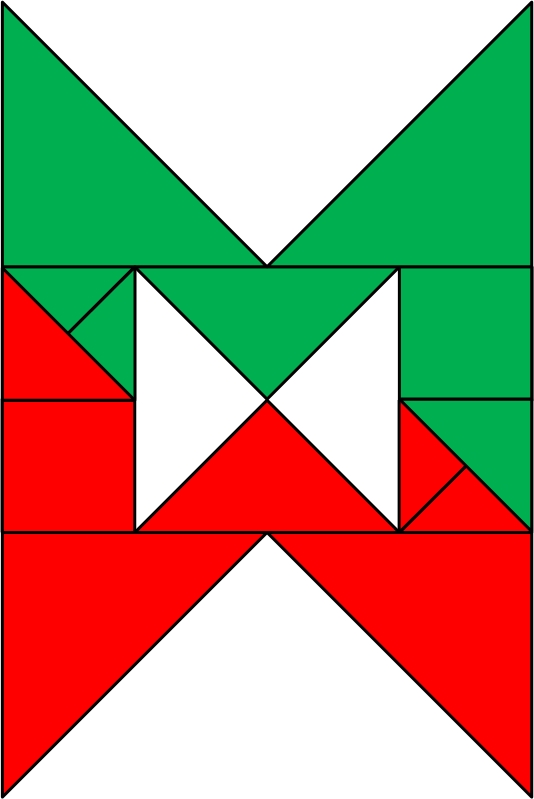
\includegraphics[width=0.25\textwidth]{wXm}
	\end{center}
	\vspace*{\fill}
\end{titlepage}


\tableofcontents
\newpage


\section{Introduction}
This domain analysis concerns combinatorial objects, along with primitive objects this kind of objects can be used to design xMAS models with the WickedXmas tool. In fact combinatorial objects are xMAS models itself but left open with unconnected ports, parameterizable and allow recursive reuse.\\
The benefits of combinatorial objects are those of re-usability, it makes complex things look simple and maintainable, it preserves correctness.\\
When designing an xMAS model in WickedXmas , the designer can make use of combinatorial objects similar as he or she does with primitive objects. Because combinatorial objects are xMAS models these can be edited just as any other kind of xMAS model except that there are unconnected ports as mentioned before.

\section{Vocabulary} 
Before we can continue explaining this matter, we need a vocabulary which make . 
\begin{itemize}
\item \textbf{WickedXmas}: Name of the tool used to design and analyse xMAS models.
\item \textbf{xMAS model}: A model based on Intel's xMAS or e\underline{x}ecutable \underline{M}icro\underline{A}rchitectural \underline{S}pecification, which is a high level design language for communication fabrics. 
\item \textbf{Primitive Object}: The xMAS language consist of eight primitive objects which are used to create xMAS models. Primitive objects are hard coded.
\item \textbf{Combinatorial Object}: A composite object which can be made of primitives and combinatorial object is an open xMAS model
\item \textbf{Channel}: A connection between an input and output port.
\item \textbf{Port}: 

\item \textbf{Initiator}: An output port.
\item \textbf{Target}: An input port.
\item \textbf{Connector}: An output port.


\end{itemize}



\section{Primitive objects}
   


\end{document} ;########################### end document ##################################;